\section{Moments}

%Lectures 7, 8, 9, 10

A moment is a force applied at a distance from a point, which causes rotation about that point. 

The distance that the force is applied from is called the \textit{moment arm}. 

\begin{figure*}[!h]
\centering
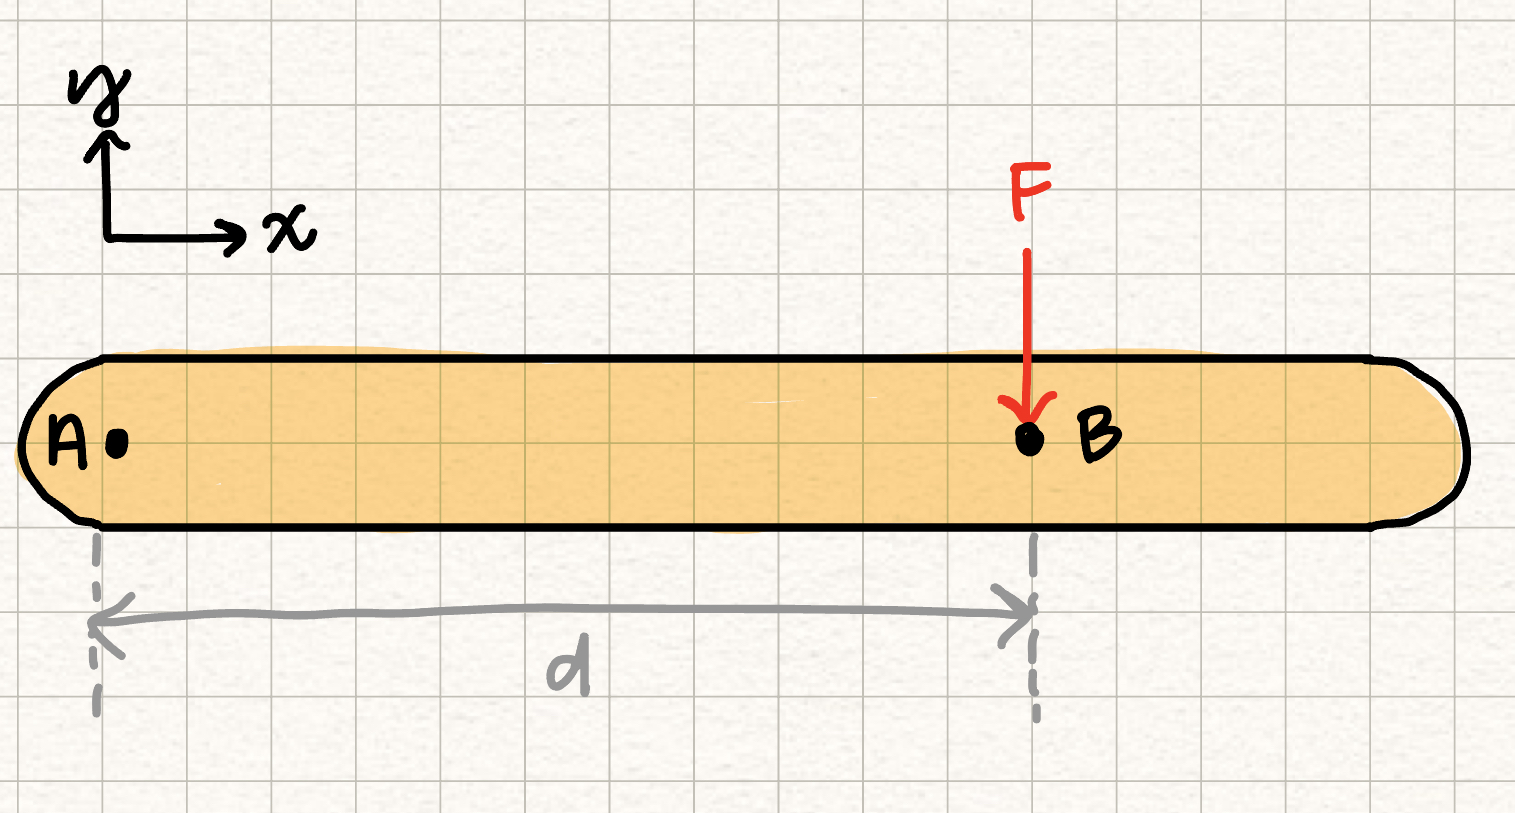
\includegraphics[angle=0, width=5in]{MomentsFigures/Moment.jpg}
\vspace{-2mm}
\caption{\small If the bar is pinned at point $A$, the force $F$, applied at a distance $d$ from point A, will cause a moment $M_A$ about point A and make the bar rotate clockwise.}
\vspace{-3mm}
\label{Fig:Moment}
\end{figure*}

The only force that produces a rotation about a point is a force perpendicular to the moment arm (in this case, the moment arm is $d$).

\blue{This could be a good place to add in example moments later in the side column for applications - could include muscle moments about a joint, oil rigs, the giant bucket that splashes water at a waterpark, pulling out a nail with a hammer.}

\subsection{Moments as scalars}

Moments can be written as scalar quantities, where 

\[{M_A} = F*d\]

Note that d is the distance from the applied force to the point of interest and that the force F is the force perpendicular to the moment arm. 

\begin{figure*}[!h]
\centering
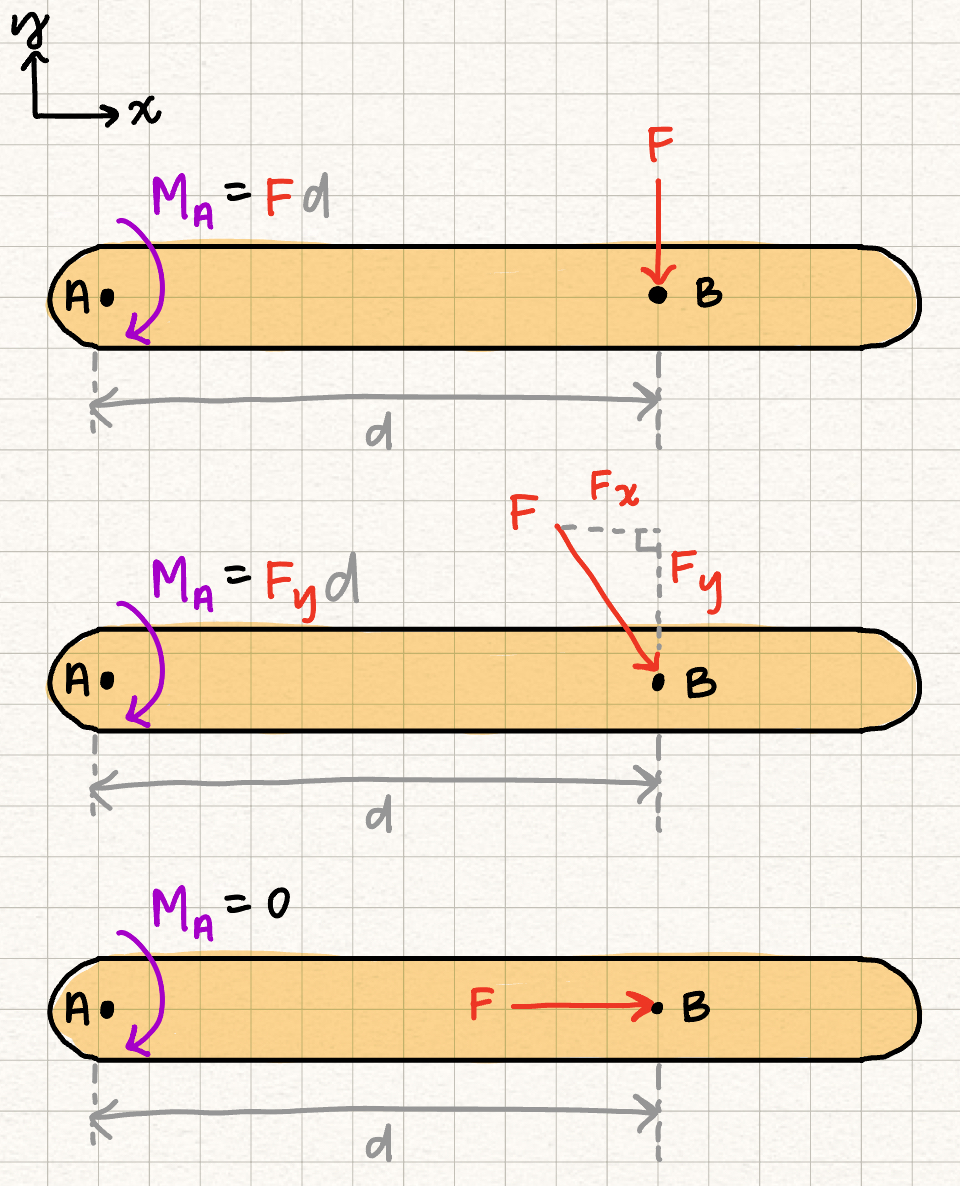
\includegraphics[angle=0, width=5in]{MomentsFigures/MomentScalar.jpg}
\vspace{-2mm}
\caption{\small The moment about point A is dependent on how much of the force $F$ is perpendicular to the moment arm $d$.}
\vspace{-3mm}
\label{Fig:MomentScalar}
\end{figure*}



You can determine the direction of moments using the right hand rule and wrapping your fingers around where the moment is turning. The direction your thumb is pointing is the direction of the moment. 

Moments are assumed to be positive when they point in the $-\hat{k}$ direction (clockwise rotation) and negative when they point in the $+\hat{k}$ direction (counterclockwise rotation). 

\begin{figure*}[!h]
\centering
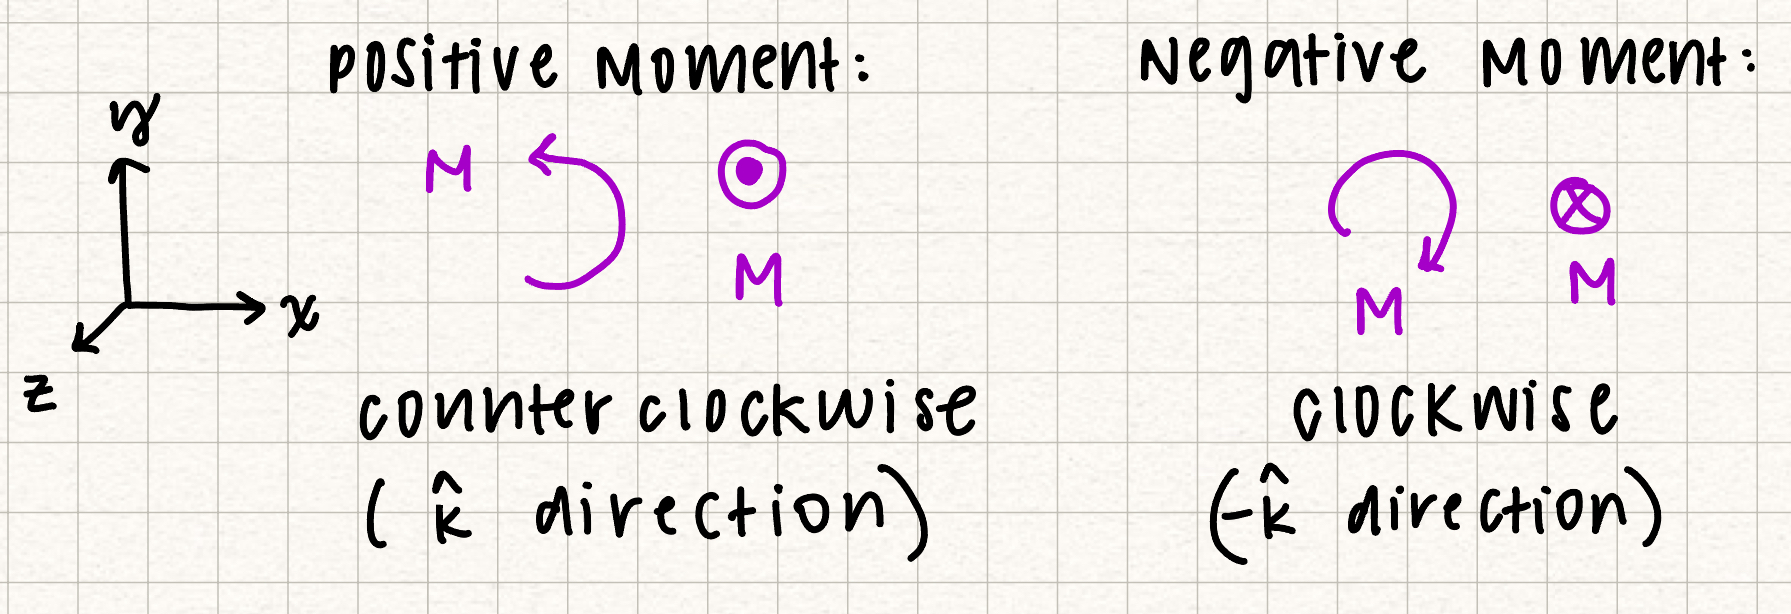
\includegraphics[angle=0, width=5in]{MomentsFigures/MomentConventions.jpg}
\vspace{-2mm}
\caption{\small Positive and negative moment conventions.}
\vspace{-3mm}
\label{Fig:MomentConventions}
\end{figure*}

%lectures 7 and 8

\subsection{Moments as vectors}

Moments can also be written as vector quantities, where the moment about point A is the cross product of the moment arm, $r$ and the force $F$. 

\[\vec{M_A} = \vec{r} \times \vec{F}\]

Using this formula, moments could have an $\hat{i}$, $\hat{j}$, and $\hat{k}$ component. 

The magnitude of the moment can be written as 

\[\vert\vec{M_A}\vert = \vert\vec{r}\vert \vert\vec{F}\vert sin\theta\]

%lectures 7 and 8

\subsection{\red{Couple Moment}}

A couple moment is a set of two equal and opposite forces with parallel lines of action that produce a moment. 

The resulting moment from a force couple can be written as 

\[M_A = F*d_{\perp}\]

where $F$ is the magnitude of one of the force vectors and d is the perpendicular distance between the two vectors. 

Note: Couple moments are independent of location when applied to a rigid body, which means the resulting moment from a force couple can be "placed" anywhere on the rigid body with the same resulting rotation from the couple moment. 

\begin{figure*}[!h]
\centering
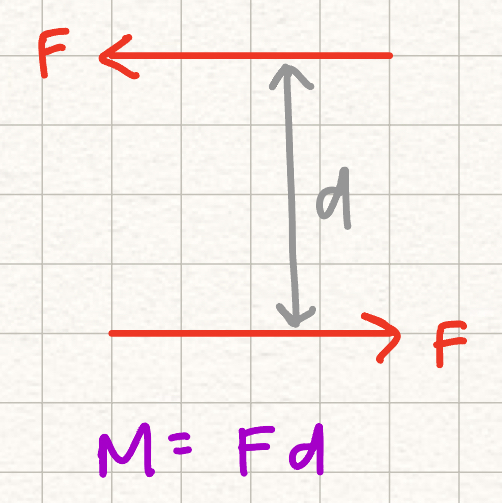
\includegraphics[angle=0, width = 2.5in]{MomentsFigures/CoupleMoment.jpg}
\vspace{-2mm}
\caption{\small A couple moment}
\vspace{-3mm}
\label{Fig:CoupleMoment}
\end{figure*}

%In vector notation, a couple moment can be written as 

%lectures 9 and 10

%\subsection{\red{Moment about an axis}}

%\red{Not sure that this needs to be a section }